\section{Kontinuerliga demonstrationer}

Under projektets gång har gruppen kontinuerligt demonstrerat produkten som utvecklats. Dessa demonstrationer har skett både för kunden och andra personer. En del av demonstrationer tillät att personerna också fick testa produkten. Demonstrationerna för kunden har innefattat både informella diskussioner kring funktioner som utvecklas, men också mer formella presentationer av produkten. Vid dessa presentationer fick kunden prova produkten och uttrycka diverse åsikter kring den. Gruppen använde denna feedback för att bestämma vilka aktiviteter som skulle fokuseras på och i sin tur få produkten att bli närmare den som önskats av kunden. 

De demonstrationer som skett för andra än kunden gav gruppen en betydligt mycket bättre insikt i hur produkten uppfattas av personer som inte är direkt associerade med detta projekt. De personer som testade hade generellt ingen koll på vad projektet innefattade eller vad produkten hade för krav. Detta resulterade i feedback som var mer fokuserad på hur produkten uppfattas av utomstående. 

Samtliga personer blev tillfrågade att fylla i en enkät efter de hade utfört ett test av produkten. Resultatet av enkäten kan ses nedan i figur \ref{fig:poll_results} och tabell \ref{tab:poll_results_table}.


\begin{figure}
    \centering
    \begin{subfigure}[]{0.5\textwidth}
        \centering
        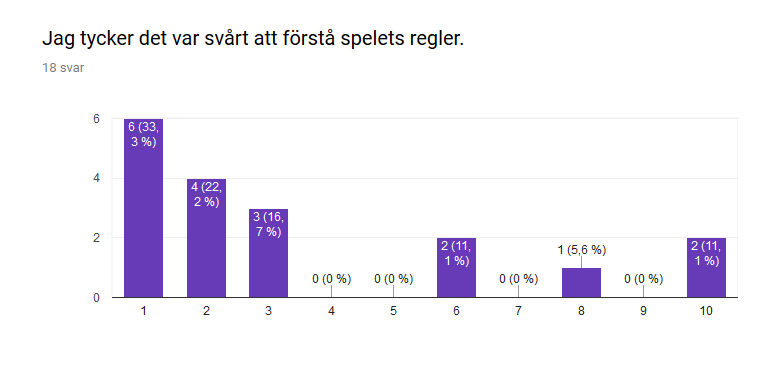
\includegraphics[width=7cm]{poll_results_2}
        \caption{}        
    \end{subfigure}%
    ~
    \begin{subfigure}[]{0.5\textwidth}
        \centering
        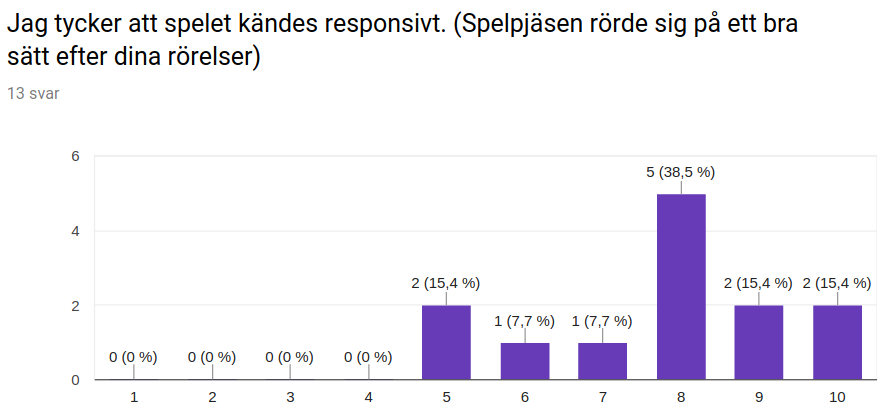
\includegraphics[width=7cm]{poll_results_3}
        \caption{}        
    \end{subfigure}

    \begin{subfigure}[]{0.5\textwidth}
        \centering
        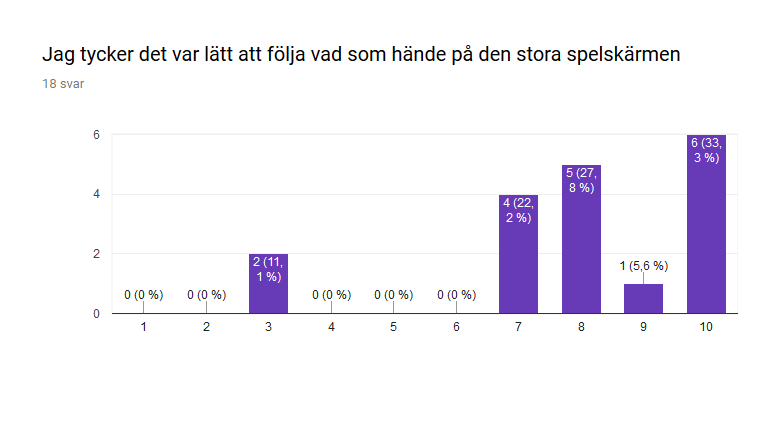
\includegraphics[width=7cm]{poll_results_4}
        \caption{}        
    \end{subfigure}%
    ~
    \begin{subfigure}[]{0.5\textwidth}
        \centering
        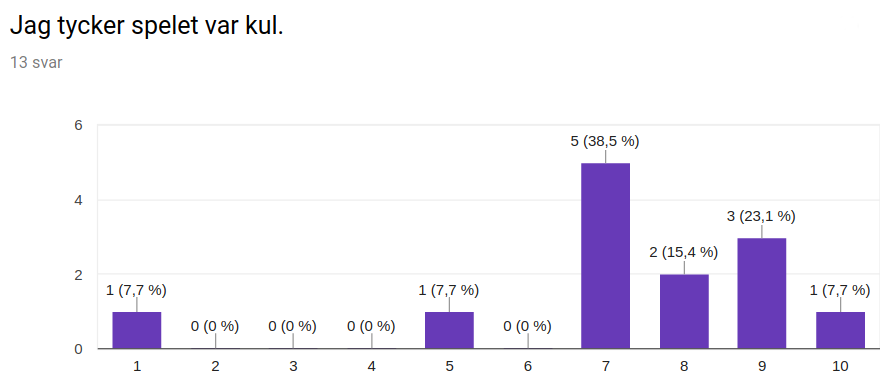
\includegraphics[width=7cm]{poll_results_5}
        \caption{}        
    \end{subfigure}

    \begin{subfigure}[]{0.5\textwidth}
        \centering
        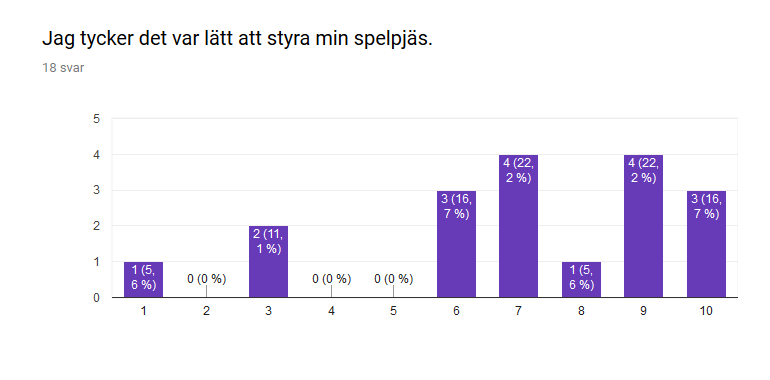
\includegraphics[width=7cm]{poll_results_6}
        \caption{}        
    \end{subfigure}%
    ~
    \begin{subfigure}[]{0.5\textwidth}
        \centering
        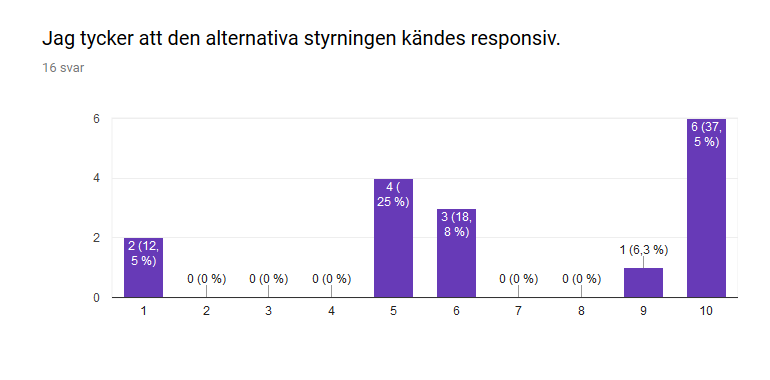
\includegraphics[width=7cm]{poll_results_7}
        \caption{}    
    \end{subfigure}
    \caption{Resultat från enkäten testpersonerna var tillfrågade att fylla i}
    \label{fig:poll_results}
\end{figure}

\begin{table}
    \centering
    \begin{tabular}{| l | l | l | l | l | l | l |}
        \cline{2-7}
        \multicolumn{1}{c|}{} & (a) & (b) & (c) & (d) & (e) & (f) \\ \hline
        Medelvärde & 4.2 & 7.8 & 7.6 & 7.2 & 6.5 & 5.8  \\ \hline
        Median & 3 & 8 & 8 & 7 & 7 & 6  \\ \hline
        Standardavvikelse & 3.4 & 1.6 & 2.4 & 2.3 & 2.8 & 3.1  \\ \hline
    \end{tabular}
    \caption{Medelvärden, median och standardavvikelse för resultaten av enkäten}
    \label{tab:poll_results_table}
\end{table}



% \begin{center}
%     \begin{tabular}{| l | l | l | l | l | l | l |}
%         \hline
%          & (a) & (b) & (c) & (d) & (e) & (f) \\ \hline
%         Medelvärde & 4.2 & 7.8 & 7.6 & 7.2 & 6.5 & 5.8 \\ \hline
%         Median & 3 & 8 & 8 & 7 & 7 & 6 \\ \hline
%         Standardavvikelse & 3.4 & 1.6 & 2.4 & 2.3 & 2.8 & 3.1 \\ \hline
%     \end{tabular}
% \end{center}

% \begin{figure}
%     \centering
%     \begin{subfigure}{0.5\textwidth}
%         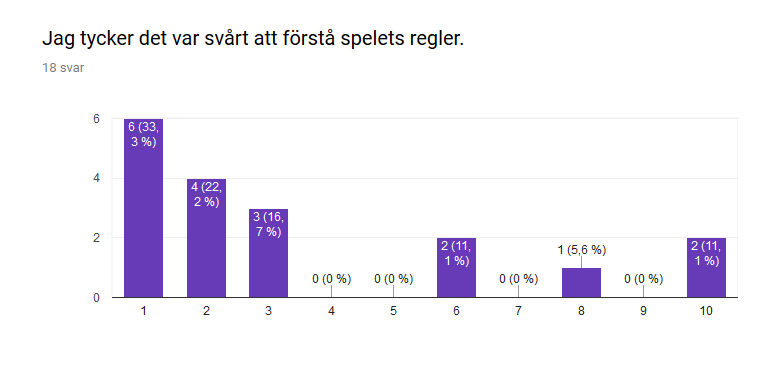
\includegraphics[width=0.4\textwidth]{poll_results_2}
%         \label{fig:poll_results_2}
%     \end{subfigure}%
%     \begin{subfigure}{0.5\textwidth}
%         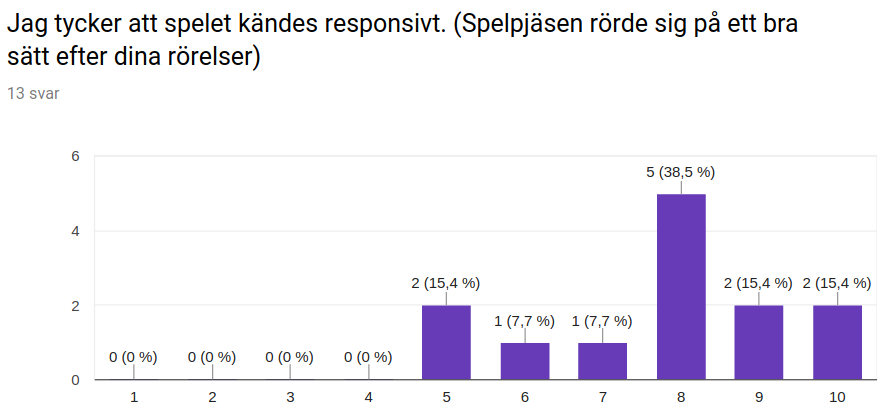
\includegraphics[width=0.4\textwidth]{poll_results_3}
%         \label{fig:poll_results_3}
%     \end{subfigure}

%     \begin{subfigure}{0.5\textwidth}
%         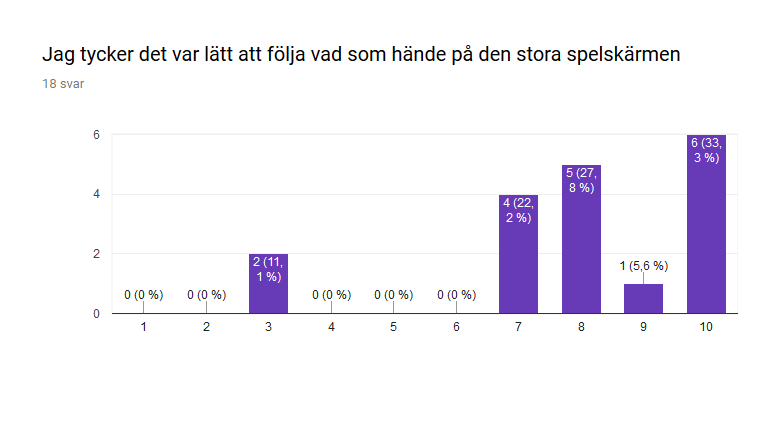
\includegraphics[width=0.4\textwidth]{poll_results_4}
%         \label{fig:poll_results_4}
%     \end{subfigure}%
%     \begin{subfigure}{0.5\textwidth}
%         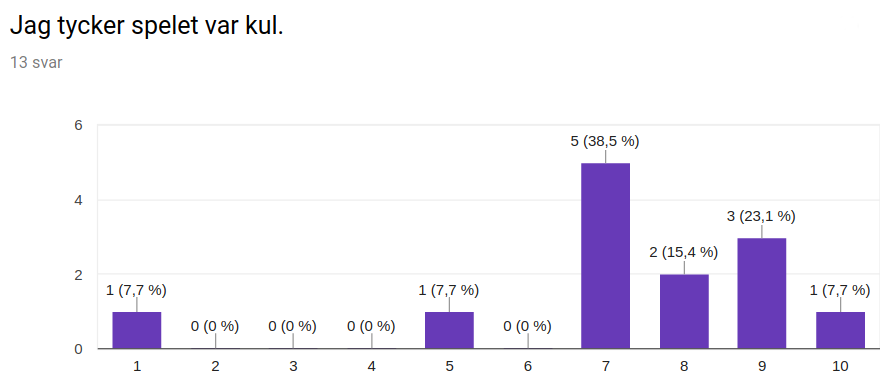
\includegraphics[width=0.4\textwidth]{poll_results_5}
%         \label{fig:poll_results_5}
%     \end{subfigure}

%     \begin{subfigure}{0.5\textwidth}
%         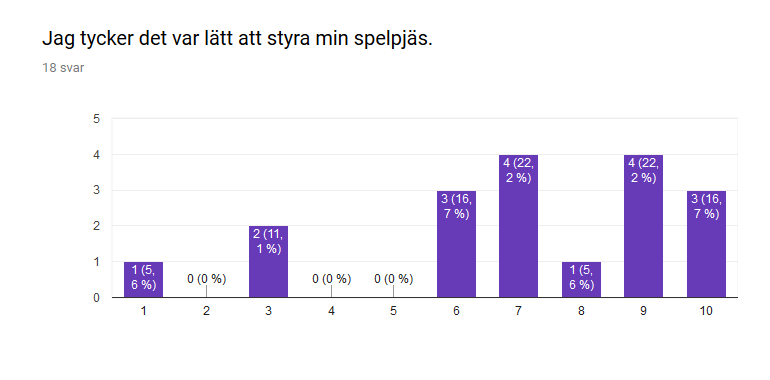
\includegraphics[width=0.4\textwidth]{poll_results_6}
%         \label{fig:poll_results_6}
%     \end{subfigure}%
%     \begin{subfigure}{0.5\textwidth}
%         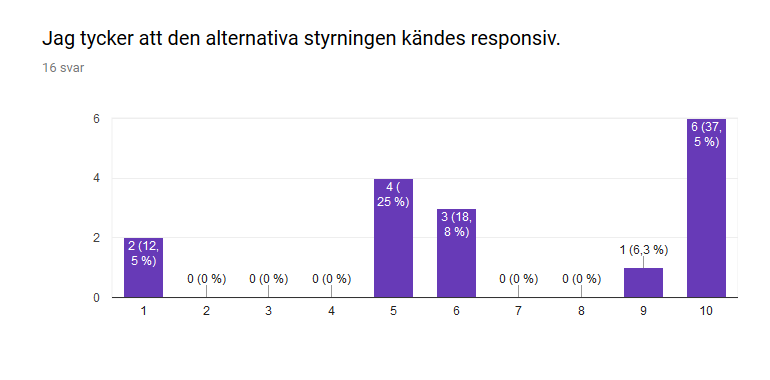
\includegraphics[width=0.4\textwidth]{poll_results_7}
%         \label{fig:poll_results_7}
%     \end{subfigure}
% \end{figure}